\documentclass[11pt]{article}
\usepackage{../EllioStyle}
\usepackage{listings}

\definecolor{codegreen}{rgb}{0,0.6,0}
\definecolor{codegray}{rgb}{0.5,0.5,0.5}
\definecolor{codepurple}{rgb}{0.58,0,0.82}
\definecolor{backcolour}{rgb}{0.95,0.95,0.92}

\graphicspath{ {imgs/} }

\title{Homework 1}
\author{Elliott Pryor}
\date{6 September 2023}

\rhead{Homework 1}
\lhead{Elliott Pryor}

\begin{document}
\maketitle

\problem{1}

Consider the system shown in Figure \ref{fig:1-1}. Derive the expression for y(t) in
terms of $y(0)$, $\dot{y}(0)$ and $f(t)$.

\begin{figure}[h] 
    \centering
    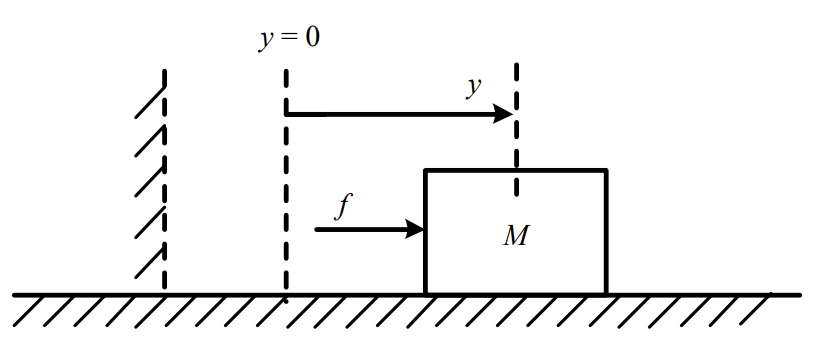
\includegraphics[width=0.55 \linewidth]{fig11.png}
    \caption{System for Problem 1,2}
    \label{fig:1-1}
\end{figure}

\soln

Without a definition of $f(t)$ we cannot do much. 
The velocity is the integral of the acceleration over time, plus the initial velocity.
Then the position is the integral of the velocity.

\begin{align}
    \ddot{y}(t) &= \frac{1}{M} f(t)\\
    \dot{y}(t) &= \dot{y}(0) + \int_0 ^t \frac{1}{M} f(k)dk  \\
    y(t) &= y(0) + \int_0 ^t \left[ \dot{y}(0) + \int_0 ^j \left( \frac{1}{M} f(k)dk \right) dj \right]
\end{align}


\problem{2}

Consider the system shown in Figure \ref{fig:1-1}. Calculate an open loop control $f(t)$
to bring $y(t)$ from $y(0) = y_0 \neq 0$ and $\dot{y}(0) = 0$ to $y(1) = 0$ and $\dot{y}(1) = 0$. 
If $M$ is reduced to $0.9M$, under the same $f(t)$, what will $y(1)$ be?

\soln

Lets pick an `easy' function for $f(t)$, so lets try to find a piecewise constant one.
We know that it needs to stop, so we want $f(t)$ to be symmetric around 0.5 (this will bring us back to the initial condition of $\dot{y}_0=0$).
We also know that it needs to arrive at the destination, so we want to make it halfway to the destination by $t=0.5$.
Thus, $\dot{y}(0.5) = 2y_0$.

\begin{figure}[h] 
    \centering
    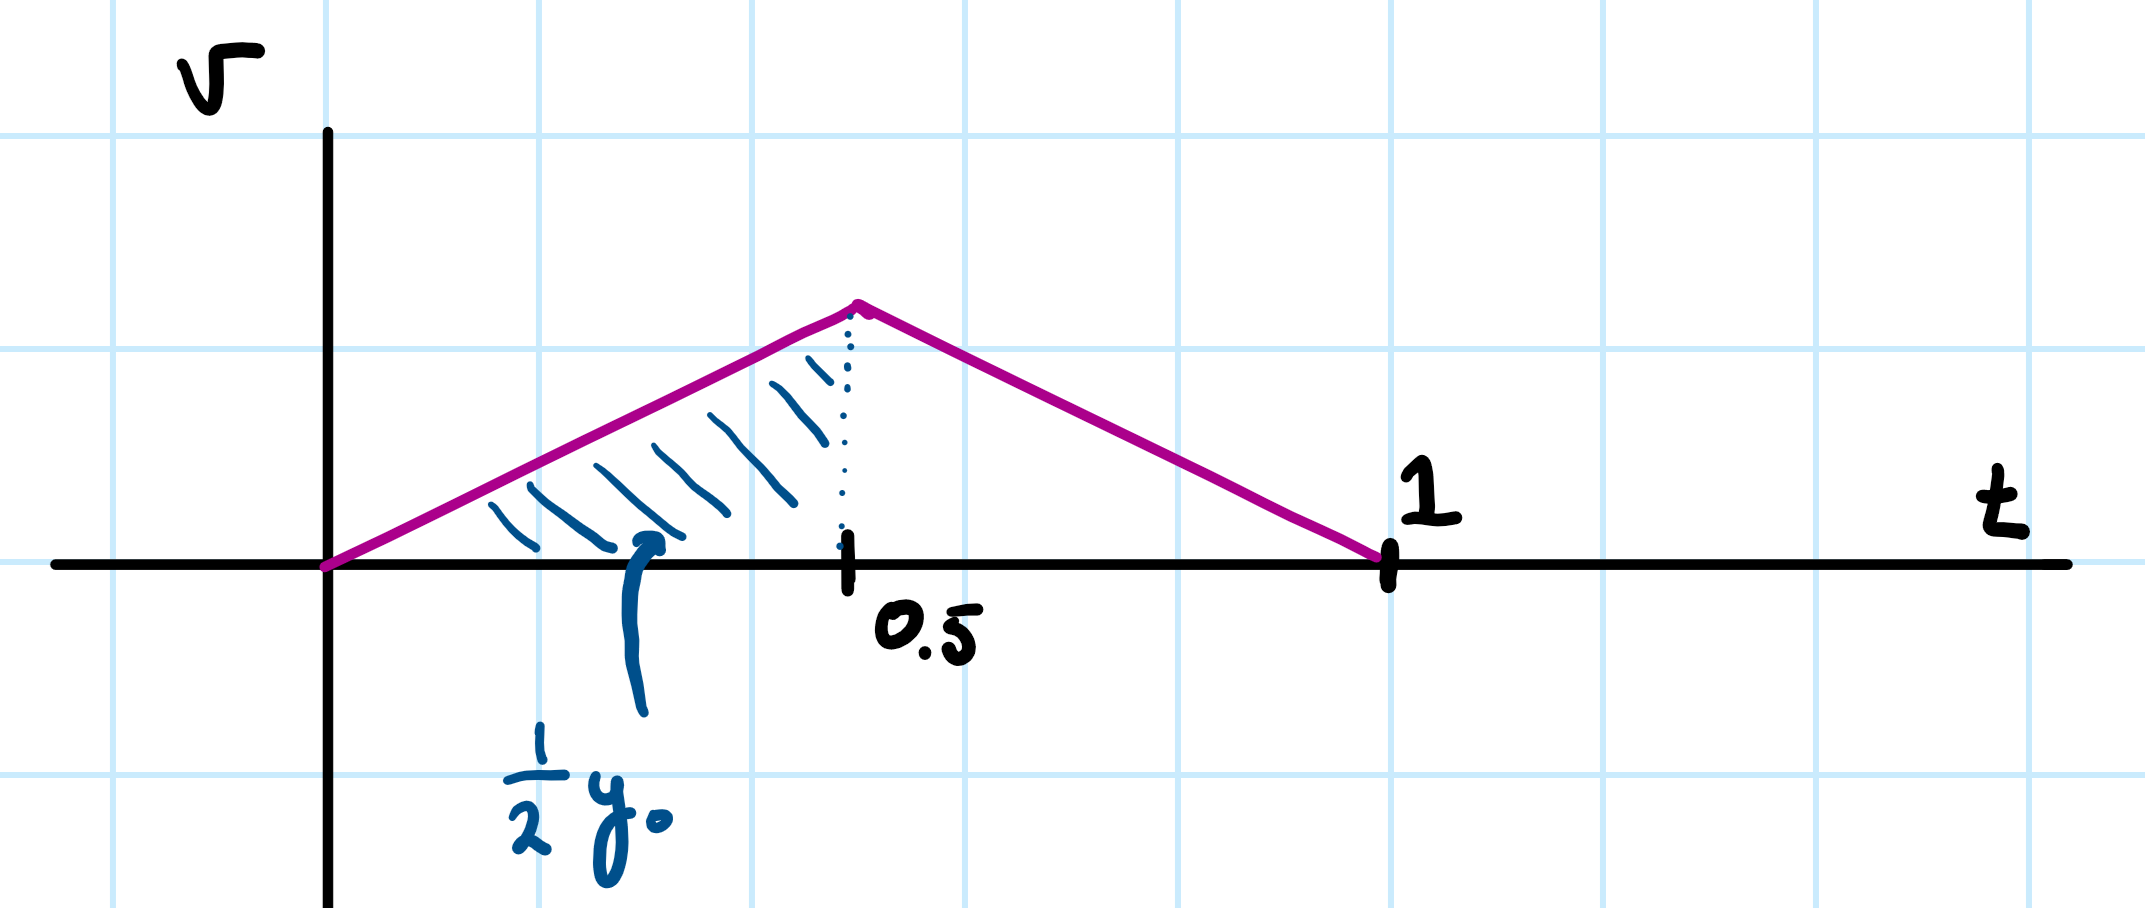
\includegraphics[width=0.55 \linewidth]{p2}
    \caption{Diagram of desired $v(t)$}
    \label{fig:p2}
\end{figure}

So then we just need to find $f$ to match this slope.
$f(t) = \begin{cases}
    -4My_0 & \text{if } t < 0.5 \\
    4My_0 & \text{if } t > 0.5 \\
\end{cases}$

This clearly satisfies the first condition that $\dot{y}(1) = 0$.
we get $\dot{y}(t) = \begin{cases}
    -4y_0 * t &\text{if } t < 0.5 \\
    4y_0 * t - 4y_0 &\text{if } t \geq 0.5
\end{cases}$
Integrating this to get the position we get
$y(t) = \begin{cases}
    y_0 - 2 y_0 t^2 &\text{if } t < 0.5 \\
    2y_0t^2 - 4y_0t + 2y_0 &\text{if } t \geq 0.5
\end{cases}$
Which satisfies $y(1)=0$ as required.

If $M$ is changed to $0.9M$ we get 
$\dot{y}(t) = \begin{cases}
    -4 \frac{10}{9} y_0 * t &\text{if } t < 0.5 \\
    4 \frac{10}{9} y_0 * t - 4 \frac{10}{9} y_0 &\text{if } t \geq 0.5
\end{cases}$,
but then\\
$y(t) = \begin{cases}
    y_0 - 2 \frac{10}{9} y_0 t^2 &\text{if } t < 0.5 \\
    \frac{20}{9} y_0t^2 - \frac{40}{9} y_0t + \frac{19}{9} y_0 &\text{if } t \geq 0.5
\end{cases}$
so $y(1) = -1/9 y_0$.

\problem{3}

Describe how you usually adjust the shower water temperature you are
comfortable with. What type of feedback do you think you are applying? What are the
actuator and sensor?

\soln

I normally increase it until it is too hot, then decrease it a bit,
then I repeat with smaller and smaller increments until it is just right.
This would be damped feedback control.

The actuator would be the temperature knob, and the sensor is my body.


\problem{4}

Identify a feedback control system that is not discussed in this chapter and
describe how feedback works in the system.

\soln

A classic control problem is the inverted pendulum.
Where the `goal' is to keep the pendulum upright.
You can design a controller that observes the pendulum angle,
then decides to move the bottom of the pendulum left or right to maintain equilibrium.

\begin{figure}[h] 
    \centering
    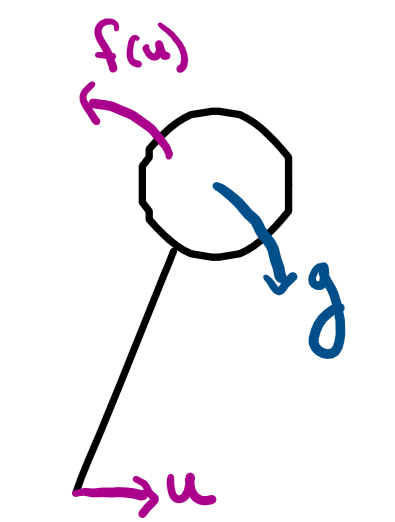
\includegraphics[width=0.35 \linewidth]{p4}
    \caption{Inverted Pendulum}
    \label{fig:p4}
\end{figure}

\problem{5}

Consider the toilet water tank, shown in Figure \ref{fig:16}. One way to reduce the
amount of water used for each flush is put a rock inside the water tank. Would this cause
the water level to rise higher when the fill valve is closed off? Give your reason.

\begin{figure}[h] 
    \centering
    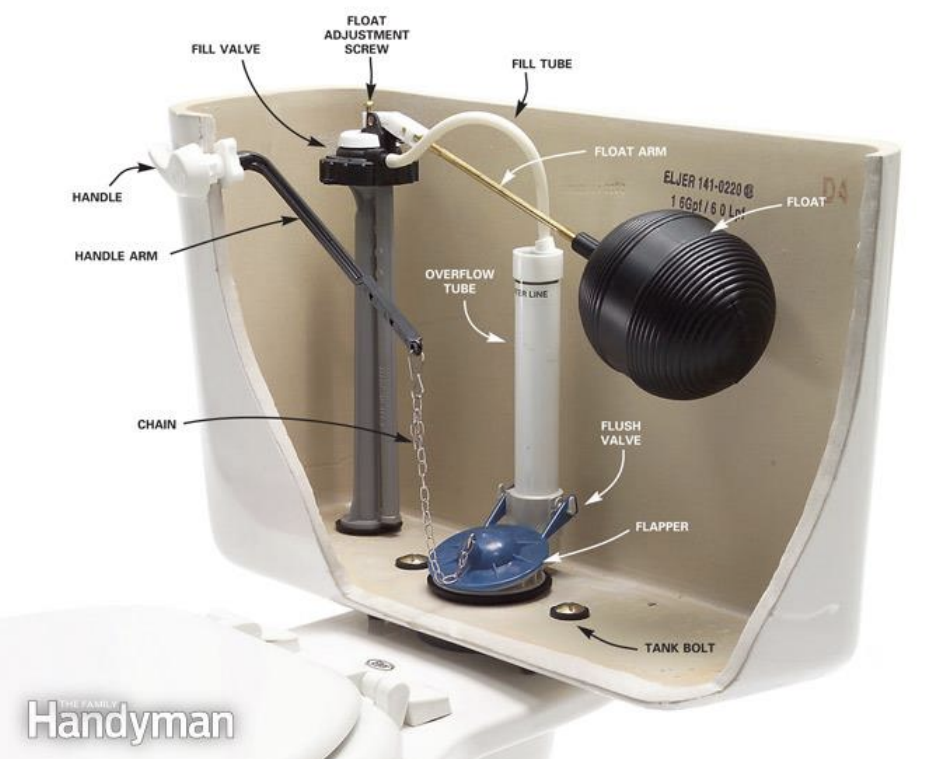
\includegraphics[width=0.55 \linewidth]{fig16.png}
    \caption{System for problem 5}
    \label{fig:16}
\end{figure}

\soln


No, it would still fill to the same level.
The sensor detects the level of water and closes the valve when it reaches the desired level.
Since this uses feedback, it would still reach the same water level regardless.

When you first put the rock in (before it is flushed the first time), the water level would be raised
due to the displacement. Many toilets have an overflow where it will drain the excess water, so that would also maintain
the proper water level for the initial flush, as it would allow the excess to drain.

\problem{6}

How would you set the desired water level in the toilet water tank, shown in
Figure \ref{fig:16}, and the desired shaft rotation speed in the Watt steam engine, shown in Fig. \ref{fig:watt}?

\begin{figure}[h]
    \centering
    \begin{subfigure}[b]{0.45\textwidth}
        \centering
        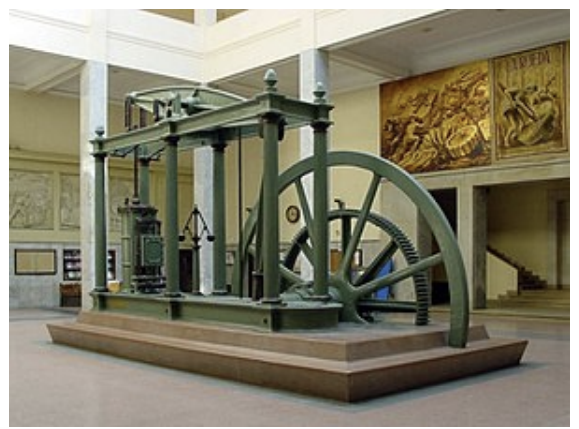
\includegraphics[width=\textwidth]{fig17}
        \label{fig:w1}
    \end{subfigure}
    \hfill
    \begin{subfigure}[b]{0.45\textwidth}
        \centering
        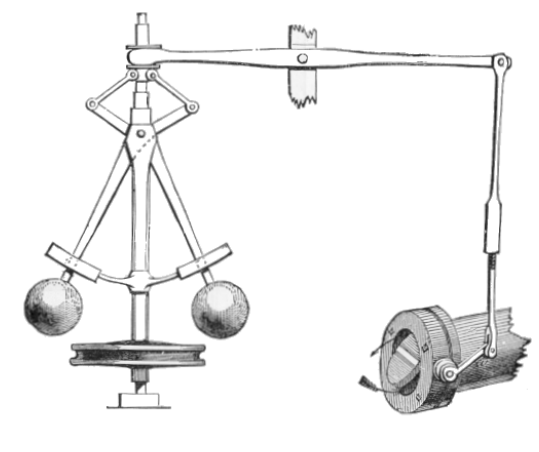
\includegraphics[width=\textwidth]{fig18}
        \label{fig:w2}
    \end{subfigure}
    \caption{Watt engine diagram}
    \label{fig:watt}
\end{figure}


\soln

For the toilet, you can adjust the float arm.
Bending it downward will make it turn off sooner.
Downward because then the float is lower so the system acts like the water level is higher than it is.
Conversely you can bend it up, to make the system act like the water level is lower than it is, and turn off later (increase fill amount).
Adjusting the height of the fill valve also does the same thing.

For the watt steam engine, you can adjust the weight of the two masses.
A heavier mass will increase the desired rotation speed (as it takes more angular velocity to sufficiently raise the masses and activate the governor).
A lighter mass will decrease the rotation speed.

\end{document}